\documentclass[12pt]{article}
\usepackage[utf8]{inputenc}
\usepackage{amsmath}
\usepackage{graphicx}
\title{CS 470 Spring 2011 \\
     Project 1A}
\author{Colby Blair}
\date{Due February 9th, 2011}
\begin{document}
\maketitle
\begin{abstract}
In Artificial Intelligence, we can test intelligent agents on their ability to navigate maps to reach a goal position. For each position, there is a choice of options that we can take, and how process these options depends on which search we choose. With each step, our new possible routes increases exponentially. The search algorithm must be able to handle all these possible routes one by one, and build routes efficiently. This report will test the Breadth First Search, discuss the methodology, and highlight the pros and cons of this type of search.
\end{abstract}
\pagebreak
\section{Breadth First Search}
\subsection{Procedure}
Consider a map like the following:
\\
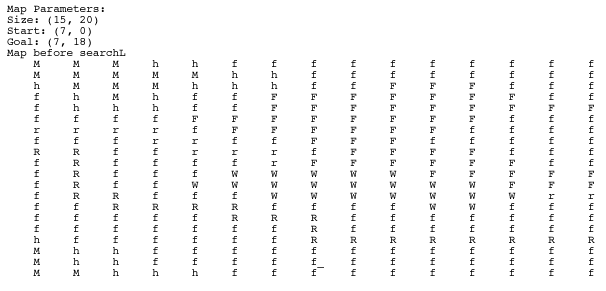
\includegraphics[width=120mm,height=60mm]{images/breadth/init_map.png}
\\
The search starts at cell x = 7, y = 0. Each cell has a cost signified by a character (R = low cost road, M = high cost mountain), but Breadth First Search does not care. It will simply find the shortest distance to the goal (there may be multiple that are equal). The only time this algorithm considers cost is when it is going off the side of the map or going into W (water), both of which have an invalid cost of 0 and are not considered.
\\ \\
This Breadth First Search uses 3 data structures: a Frontier Queue, an Explored List, and a Value Matrix. The only technical notes past these is that the Value Matrix is a matrix (or 2 dimensional array) of 'node' classes. Each 'node' class has members name, val, x, and y (where val equals the cost of the cell). Value\_Matrix[0][0] then equals node('M',10,0,0), etc. Later we will see that each cell node also has a node parent pointer, but ignore this for now.
 
\pagebreak
 
Let's consider our start section of the map:
\begin{center} 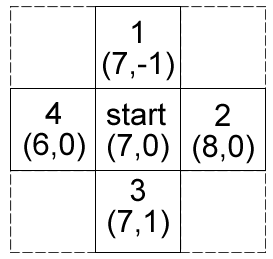
\includegraphics[width=60mm]{images/breadth/init_pos.png} \end{center}
Cells above are labeled in the order the algorithm adds them to a queue.
\begin{enumerate}
\item 'start' is added.
\item while the front of the queue is not the goal:
\begin{enumerate}
 \item front's neighbors are added to the end of the queue
 \item front is popped from the queue
\end{enumerate}
\end{enumerate}
So each iteration would look something like the following:
\\ \\
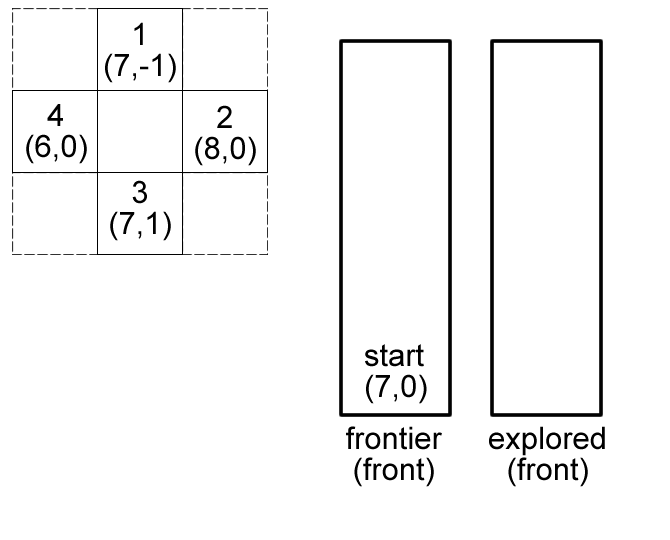
\includegraphics[width=60mm]{images/breadth/pos01.png}
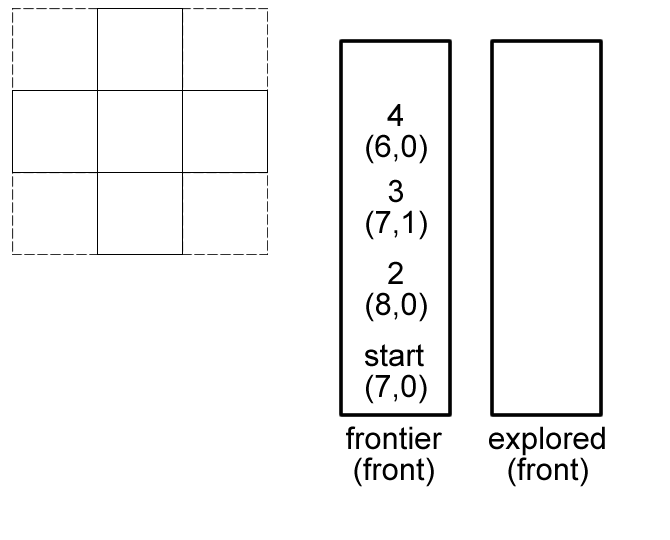
\includegraphics[width=60mm]{images/breadth/pos02.png}
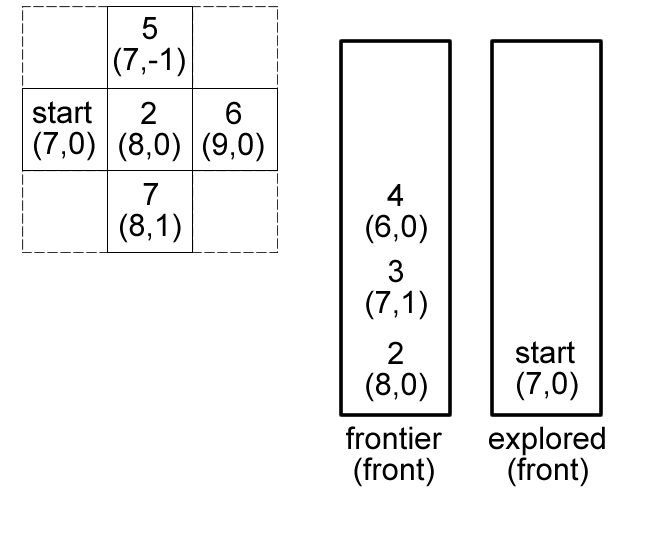
\includegraphics[width=60mm]{images/breadth/pos03.png}
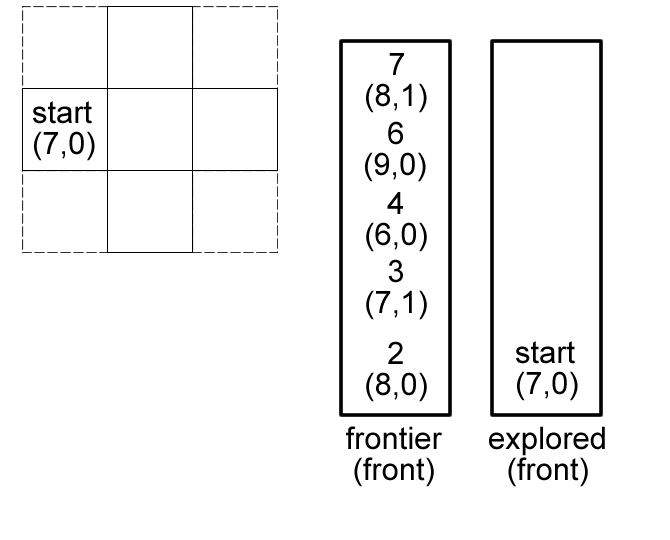
\includegraphics[width=60mm]{images/breadth/pos04.png}
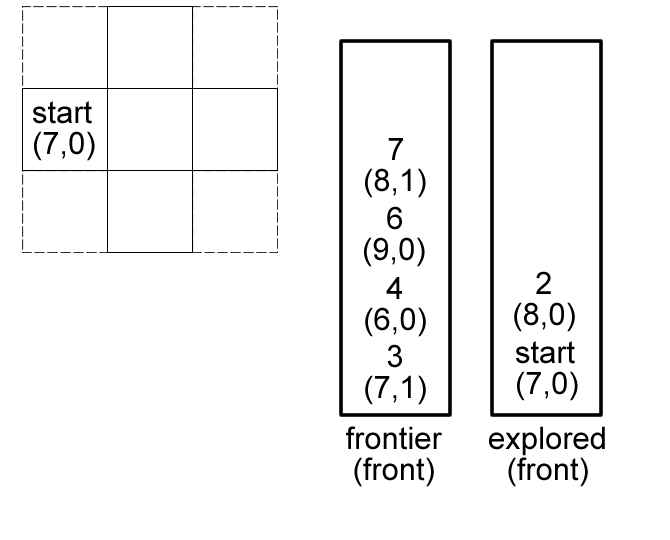
\includegraphics[width=60mm]{images/breadth/pos05.png}
\\
This would continue on until the node (or cell) on the front of frontier queue was the goal. Notice that the search does not add nodes outside the bounds of the map or matrix (i.e. nodes 1 and 5 above). Also, nodes (or cells) that already exist in the explored list are not re-added to the frontier list.
\subsection{Procedure Summary}
This search is called a Breadth First Search because at every cell, there is a decision tree of possible new cells to move to. When the search processes every neighbor cell first before processing those neighbor cells' neighbors, the search has covered the breadth of the top level of the decision tree before moving on. In contrast, if the search was at the 'start' cell, processed cell 3 from above, and then processed all of cell 3's neighbors before looking at cell 4, the search would be searching as a Depth First Search.
\\ \\
The Depth First search would be searching each possible 1st neighbor until the last possible neighbor, and then backing up from the bottom of the decision tree. Cell 4 above wouldn't get considered until every possible path from cell 3 was exhausted with no route to the goal.
\subsection{Path Tracing}
An extra feature to searching is to trace the path an individual took to get to the location. There are several ways to do this. The way the search did this here is each node on the Value Matrix had a Parent Pointer. This pointer was set to Null initially. Then, whenever a node (or cell) was added to the frontier queue, the corresponding cell node on the Value Matrix had its parent pointer set to the corresponding Value Matrix cell node
of the node that added.
\\ \\
For example, in the figures above, when cell node 'start' added cell node 3 to the frontier queue, Value Matrix cell node 3's parent was set to Value Matrix cell node 'start'. Since cell node 3 could only ever be added once, it will only ever have its parent set once. Thus, a route back to the cell node 'start' will always be found anywhere in the explored Value Matrix.
\subsection{Completeness, Efficiency, and Complexity}
The Breadth First Search is a complete search, meaning it will find the goal if one exists. It will also find the shallowest solution in the decision tree. The Time Complexity (or time it takes to find the goal) is $\approx B^{d}$, or about the number of each neighbor a cell could have to the power of the max depth of the decision tree. The Space Complexity (memory used, or storage all new neighbors to the frontier queue) is $\approx B^{d}$.
\\ \\
This search is advantageous to the Depth First Search, which is only sometimes complete (only when the depth is finite). This search will also find the shallowest solution (shortest path), which is not gaurenteed or even likely for Depth First Search. Depth first search will almost always have less Time Complexity (quicker) with an upper bound of $B^{d}$, and will have less Space Complexity (uses less memory). In practicality, very big maps would have to use Depth First Search for the Complexity reasons.
\pagebreak
\subsection{Program Output}
The final output of the Breadth First Search is:
\\
\begin{center}
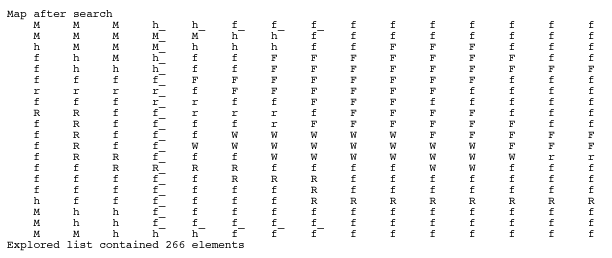
\includegraphics[width=120mm,height=60mm]{images/breadth/final_breadth_map.png}
\end{center}
We can see that this search takes the straightest path over until the 'W' water barrier is out of the way. The search goes straight down towards the goal, and then once parallel, cuts straight back across. This is the shortest path on our discrete map of cells. It is in now way the least cost path, but it is the straightest, considering the impassable 'W' water barrier.
\subsection{Conclusion}
The Breadth First Search found the straightest path, but at a high Space Complexity / memory price. The frontier explored list contained 266 cell nodes, the majority of the 15 x 20 map (300 cell nodes). This Space Complexity on a larger map could be a big issue, and a different search algorithm may be needed.
\end{document}
